% ------------------------------------------------------------------------------
% TYPO3 CMS 6.2 LTS - What's New - Chapter "Responsive Images" (Russian Version)
%
% @author	Andrey Aksenov <aksenovaa@bk.ru>
% @license	Creative Commons BY-NC-SA 3.0
% @link		http://typo3.org/download/release-notes/whats-new/
% @language	Russian
% ------------------------------------------------------------------------------
% Chapter: Responsive Images
% ------------------------------------------------------------------------------

\section{Responsive Images - адаптивные изображения}
\begin{frame}[fragile]
	\frametitle{Responsive Images - адаптивные изображения}

	\begin{center}\huge{Глава 2:}\end{center}
	\begin{center}\huge{\color{typo3darkgrey}\textbf{Responsive Images}}\end{center}
	\begin{center}\huge{\color{typo3darkgrey}\textbf{(адаптивные изображения)}}\end{center}

\end{frame}

% ------------------------------------------------------------------------------
% Select Screen Size In Page Preview
% ------------------------------------------------------------------------------

\begin{frame}[fragile]
	\frametitle{Responsive Images - адаптивные изображения}
	\framesubtitle{Выберете размер экрана в предварительном просмотре}

	\begin{itemize}
		\item В меню "Просмотр" (View) можно выбрать разные размеры экрана для тестирования адаптивных (responsive) сайтов
	\end{itemize}

	\begin{figure}
		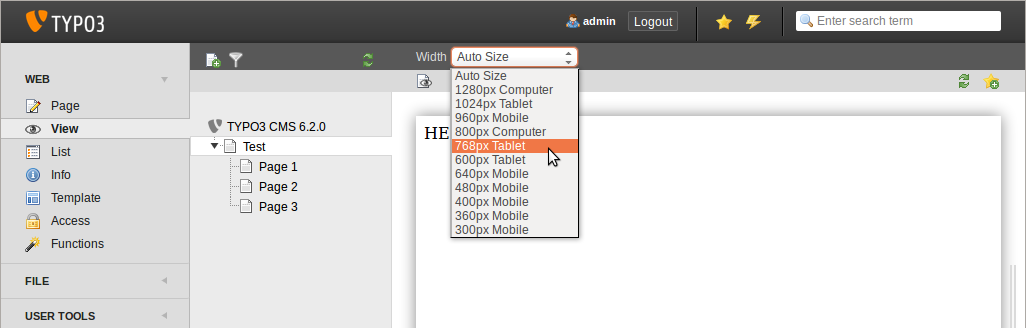
\includegraphics[width=0.95\linewidth]{Images/ResponsiveImages/ScreenSizeInPagePreview.png}
	\end{figure}

\end{frame}

% ------------------------------------------------------------------------------
% Customize Available Screen Sizes
% ------------------------------------------------------------------------------

\begin{frame}[fragile]
	\frametitle{Responsive Images - адаптивные изображения}
	\framesubtitle{Настройка доступных размеров экрана}

	\begin{itemize}
		\item Размеры экрана настраиваются через PageTSconfig:

		\lstset{
			basicstyle=\fontsize{7}{9}\selectfont\ttfamily
		}

		\begin{lstlisting}
			mod.web_view.previewFrameWidths {
			  1780.label = <any LLL or string>
			  1780.height = 145
			}
		\end{lstlisting}

		\item Ширина определяется ключом (здесь: 1780), высота не обязательна
		\item Предопределенные размеры можно найти в файле:\newline
			\small\texttt{typo3/sysext/core/Configuration/DefaultConfiguration.php}\normalsize
		\item Метки можно определить через PageTSconfig:

		\begin{lstlisting}
			mod.web_view.previewFrameWidths {
			  1280.label = LLL:EXT:viewpage/Resources/Private/Language/locallang.xlf:computer
			  1024.label = LLL:EXT:viewpage/Resources/Private/Language/locallang.xlf:tablet
			}
		\end{lstlisting}

	\end{itemize}

\end{frame}

% ------------------------------------------------------------------------------
% Responsive Image Galleries
% ------------------------------------------------------------------------------

\begin{frame}[fragile]
	\frametitle{Responsive Images - адаптивные изображения}
	\framesubtitle{Адаптивные галереи изображений}

	\begin{itemize}
		\item Дополнительные атрибуты для адаптивных галерей изображений
		\item "CSS styled content" дополнен для этих целей
		\item Пример: HTML5 (требует \texttt{config.doctype = html5})\newline

			TYPO3 CMS < 6.2:

			\lstset{
				basicstyle=\fontsize{7}{9}\selectfont\ttfamily
			}

			\begin{lstlisting}
				<div class="csc-textpic-imagewrap">...</div>
			\end{lstlisting}

			TYPO3 CMS >= 6.2:

			\begin{lstlisting}
				<div class="csc-textpic-imagewrap"
				  data-csc-images="{register:imageCount}"
				  data-csc-cols="{field:imagecols}">...</div>
			\end{lstlisting}

	\end{itemize}

\end{frame}

% ------------------------------------------------------------------------------
% Responsive Image Rendering
% ------------------------------------------------------------------------------

\begin{frame}[fragile]
	\frametitle{Responsive Images - адаптивные изображения}
	\framesubtitle{Вывод адаптивных изображений}

	\begin{itemize}
		\item cObject IMAGE формирует так называемый "sourceCollection" - набор исходников, для поддержки разных размеров экрана
		\item Формирование адаптивных изображений для cObjects "text/image" и "image" требует двух настроек в Редакторе констант:

			\texttt{styles.content.imgtext.responsive}\newline
			\texttt{styles.content.imgtext.layoutKey}

		\item действенные ("из коробки") варианты следующие:

			\begin{itemize}
				\item \texttt{default}:	\tabto{2cm} default \texttt{<img>}-тег
				\item \texttt{srcset}:	\tabto{2cm} \texttt{<img>}-тег с альтернативными источниками в виде атрибута srcset
				\item \texttt{picture}:	\tabto{2cm} \texttt{<picture>}-тег со вложенными тегами источниками
				\item \texttt{data}:	\tabto{2cm} \texttt{<img>}-тег с альтернативными источниками в виде атрибута data
			\end{itemize}

	\end{itemize}

\end{frame}

% ------------------------------------------------------------------------------
% Property: layoutKey
% ------------------------------------------------------------------------------

\begin{frame}[fragile]
	\frametitle{Responsive Images - адаптивные изображения}
	\framesubtitle{Свойство: layoutKey}

	\begin{itemize}
		\item \texttt{layoutKey} определяет визуализацию шаблона\newline
			(это код HTML для тега \texttt{<img>})
		\item каждый параметр показывает уникальное поведение для формирования HTML
		\item параметр \texttt{default} формирует обычный тег \texttt{<img>}\newline
			(это в случае не адаптивного сайта)
		\item Применение адаптивного шаблона требует изображений разных размеров для разных разрешений и размеров экранов
		\item В зависимости от технологии (framework) HTML, совместимости с браузерами и библиотеки JavaScript (для выбора
		нужного разрешения):

			\begin{itemize}
				\item воспользуйтесь одним из предопределенных макетов, либо
				\item создайте свой
			\end{itemize}

	\end{itemize}

\end{frame}

% ------------------------------------------------------------------------------
% Property: layout
% ------------------------------------------------------------------------------

\begin{frame}[fragile]
	\frametitle{Responsive Images - адаптивные изображения}
	\framesubtitle{Свойство: layout}

			\lstset{
				basicstyle=\tiny\ttfamily
			}

	\begin{lstlisting}
		layoutKey = {$styles.content.imgtext.layoutKey}
		layout {
		  default {
		    element = <img src="###SRC###" width="###WIDTH###" height="###HEIGHT###" ###PARAMS###
		      ###ALTPARAMS### ###BORDER######SELFCLOSINGTAGSLASH###>
		  }
		  srcset {
		    element = <img src="###SRC###" srcset="###SOURCECOLLECTION###" ###PARAMS###
		      ###ALTPARAMS### ###SELFCLOSINGTAGSLASH###>
		    source = |*|###SRC### ###SRCSETCANDIDATE###,|*|###SRC### ###SRCSETCANDIDATE###
		  }
		  picture {
		    element = <picture>###SOURCECOLLECTION###<img src="###SRC###" ###PARAMS###
		      ###ALTPARAMS######SELFCLOSINGTAGSLASH###></picture>
		    source = <source src="###SRC###" media="###MEDIAQUERY###"###SELFCLOSINGTAGSLASH###>
		  }
		  data {
		    element = <img src="###SRC###" ###SOURCECOLLECTION### ###PARAMS###
		      ###ALTPARAMS######SELFCLOSINGTAGSLASH###>
		    source = data-###DATAKEY###="###SRC###"
		  }
		}
	\end{lstlisting}

\end{frame}

% ------------------------------------------------------------------------------
% Property: layout.[layoutKey].element
% ------------------------------------------------------------------------------

\begin{frame}[fragile]
	\frametitle{Responsive Images - адаптивные изображения}
	\framesubtitle{Свойство: layout.[layoutKey].element}


	\begin{itemize}
			\item \lstinline!###SRC###!\newline
				URL для атрибута: \texttt{src}

			\item \lstinline!###WIDTH###!\newline
				Ширина изображения (в пикселях) для атрибута: \texttt{width}

			\item \lstinline!###HEIGHT###!\newline
				Высота изображения (в пикселях) для атрибута: \texttt{height}

			\item \lstinline!###PARAMS###!\newline
				Дополнительные параметры, как определено в cObject IMAGE

			\item \lstinline!###ALTPARAMS###!\newline
				Дополнительные альтернативные параметры, как определено в cObject IMAGE

	\end{itemize}

\end{frame}

% ------------------------------------------------------------------------------
% Property: layout.[layoutKey].element
% ------------------------------------------------------------------------------

\begin{frame}[fragile]
	\frametitle{Responsive Images - адаптивные изображения}
	\framesubtitle{Свойство: layout.[layoutKey].element}

		\begin{itemize}
			\item \lstinline!###BORDER###!\newline
				Рамка (в пикселях) для атрибута: \texttt{border}

			\item \lstinline!###SELFCLOSINGTAGSLASH###!\newline
				Закрытый тег, например \texttt{<img ... />}, а не \texttt{<img ... >}\newline
				(зависит от \texttt{config.xhtmlDoctype} либо \texttt{config.doctype})

			\item \lstinline!###SOURCECOLLECTION###!\newline
				Дополнительные исходные изображения, в зависимости от применяемого адаптивного дизайна.
				Точные значения определяются в ключе: \texttt{layout.[layoutKey].source}

	\end{itemize}

\end{frame}

% ------------------------------------------------------------------------------
% Property: sourceCollection.[dataKey]
% ------------------------------------------------------------------------------

\begin{frame}[fragile]
	\frametitle{Responsive Images - адаптивные изображения}
	\framesubtitle{Свойство: sourceCollection.[dataKey]}

	\begin{itemize}
		\item sourceCollection по умолчанию для EXT:css\_styled\_content
		\item крайне рекомендуется написание собственной sourceCollection

			\lstset{
				basicstyle=\tiny\ttfamily
			}

			\begin{lstlisting}
				sourceCollection {
				  small {
				    width = 200
				    srcsetCandidate = 600w
				    mediaQuery = (max-device-width: 600px)
				    dataKey = small
				  }
				  smallRetina {
				    if.directReturn = 1
				    width = 200
				    pixelDensity = 2
				    srcsetCandidate = 600w 2x
				    mediaQuery = (max-device-width: 600px) AND (min-resolution: 192dpi)
				    dataKey = smallRetina
				  }
				}
			\end{lstlisting}
	\end{itemize}

\end{frame}

% ------------------------------------------------------------------------------
% Further Resources (External Links)
% ------------------------------------------------------------------------------

\begin{frame}[fragile]
	\frametitle{Responsive Images - адаптивные изображения}
	\framesubtitle{Дополнительные ресурсы}

	\begin{itemize}
		\item Рабочий пример кода на:\newline
			\small\url{http://wiki.typo3.org/Responsive_Image_Rendering}\normalsize

		\item Статья Sven Wolfermann на typo3.org:\newline
			\small\url{http://typo3.org/news/article/responsive-image-rendering-in-typo3-cms-62/}\normalsize

		\item Рабочий проект "Responsive Image Community Group":\newline
			\small\url{http://responsiveimages.org}\normalsize

	\end{itemize}

\end{frame}

% ------------------------------------------------------------------------------

